\documentclass[a4paper,12pt,Times]{article}
\usepackage{abakos}  %pacote com padrão da Abakos baseado no padrão da PUC

%%%%%%%%%%%%%%%%%%%%%%%%%%%
%Capa da revista
%%%%%%%%%%%%%%%%%%%%%%%%%%

%\setcounter{page}{80} %iniciar contador de pagina de valor especificado
\newcommand{\monog}{Análise Comparativa de Métodos para Identificação de Pontes: Abordagens Naïve e Tarjan Aplicadas ao Algoritmo de Fleury}
\newcommand{\monogES}{Comparative Analysis of Methods for Bridge Identification: Naïve and Tarjan Approaches Applied to Fleury's Algorithm}
\newcommand{\tipo}{Artigo }  % Especificar a seção tipo do trabalho: Artigo, Resumo, Tese, Dociê etc
\newcommand{\origem}{Brasil}
\newcommand{\editorial}{\textbf{Abakos}, Belo Horizonte,v. 1, n. 1, p. 00-00, Nov. 2024 - ISSN: 2316-9451}  % p. xx-xx – páginas inicial-final do artigo
% \newcommand{\lcc}{\scriptsize{Licença Creative Commons Attribution-NonCommercial-NoDerivs 3.0 Unported}}

%%%%%%%%%%%%%%%%%INFORMAÇÕES SOBRE AUTOR PRINCIPAL %%%%%%%%%%%%%%%%%%%%%%%%%%%%%%%
\newcommand{\AutorA}{Luca Ferrari Azalim}
\newcommand{\funcaoA}{}
\newcommand{\emailA}{lucaazalim@gmail.com}
\newcommand{\cursA}{Graduação em Engenharia de Software PUC Minas}
% 

\newcommand{\AutorB}{Fernando Antônio Ferreira Ibrahim}
\newcommand{\funcaoB}{}
\newcommand{\emailB}{fernandofibrahim@gmail.com}
\newcommand{\cursB}{Graduação em Engenharia de Software PUC Minas}
% 
% \newcommand{\AutorC}{Giovanni Candido da Silva}
% \newcommand{\funcaoC}{Bacharel em Sistemas de Informação}
% \newcommand{\emailC}{giovanni@pucminas.br}
% \newcommand{\cursC}{Instituto de Ciências Exatas e de Informática da PUC Minas}

% Definir macros para o nome da Instituição, da Faculdade, etc.
\newcommand{\univ}{Pontifícia Universidade Católica de Minas Gerais}

\newcommand{\keyword}[1]{\textsf{#1}}

\begin{document}
% %%%%%%%%%%%%%%%%%%%%%%%%%%%%%%%%%%
% %% Pagina de titulo
% %%%%%%%%%%%%%%%%%%%%%%%%%%%%%%%%%%

\begin{flushleft}

\begin{minipage} [c][5cm][b]{16.5cm} % a primeira minipágina tem uma altura de 1.5cm e uma largura de 2.3cm.
% comando que introduz o logo da escola que nesta altura já terá de estar na pasta imagens que 
%por sua vez está na pasta onde se guardou o arquivo tex. E introduzimos essa imagem com a mesma altura da minipage.

\includegraphics[scale=1.1]{figuras/pucmg.png} 
\end{minipage}

 \vspace{0cm} {
 \singlespacing \Large{\monog \symbolfootnote[1]{Artigo apresentado à Revista Abakos} \\ }
  \normalsize{\monogES}
 }
\end{flushleft}
\begin{flushright}
\singlespacing 
\normalsize{\AutorA \footnote{\funcaoA \cursA, \origem -- \emailA }} \\
\normalsize{\AutorB \footnote{\funcaoB \cursB, \origem -- \emailB}} \\
% \normalsize{\AutorB \footnote{\funcaoB, E-mail:\emailB \\ \cursB, \origem. }} \\
% \normalsize{\AutorC \footnote{\funcaoC, E-mail:\emailC \\ \cursC, \origem. }} \\
% \normalsize{\AutorD \footnote{\funcaoD \\ Pais de origem: \origemD. E-mail: \emailD}} \\
%deixar com o valor `0` e usar o '*' no inicio da frase
% \symbolfootnote[0]{Artigo recebido em 10 de julho de 1983 e aprovado em 29 de maio 2012}
\end{flushright}
\thispagestyle{empty}
\begin{abstract}
\noindent
O presente trabalho tem como objetivo implementar um algoritmo para a identificação de trajetos e ciclos eulerianos em grafos, com foco na comparação de diferentes métodos para a identificação de pontes. Serão consideradas as implementações dos métodos \textit{naïve} e \textit{Tarjan}, que são fundamentais para a execução do algoritmo de Fleury, escolhido devido à sua popularidade e baixa complexidade computacional. O estudo visa avaliar a eficiência de ambos os métodos na identificação de pontes, elemento crucial para a construção de trajetos e ciclos eulerianos. Espera-se que este projeto contribua para uma melhor compreensão da performance de diferentes abordagens na solução de problemas relacionados à teoria dos grafos e à otimização de rotas.
\\\textbf{\keyword{Palavras-chave: }} Caminho euleriano, Ciclo euleriano, Algoritmo de \textit{Fleury}, Identificação de pontes, Teoria dos grafos, Comparação de métodos.
\end{abstract}

%%%%%%%%%%%%%%%%%%%%%%%%%%%%%%%%%%%%%%%%%%%%%%%%%%%%%%%%%
\newpage 
\selectlanguage{english}
\begin{abstract}
\noindent
This paper aims to implement an algorithm for identifying Eulerian paths and cycles in graphs, with an emphasis on comparing different methods for bridge identification. The \textit{naïve} and \textit{Tarjan} methods will be considered, as they are key components for the execution of \textit{Fleury's} algorithm, chosen for its popularity and low computational complexity. The study seeks to evaluate the efficiency of both methods in identifying bridges, a crucial element for constructing Eulerian paths and cycles. It is expected that this project will contribute to a better understanding of the performance of different approaches in solving graph theory problems and optimizing routes.
\\\textbf{\keyword{Keywords: }} Eulerian path, Eulerian cycle, Fleury's algorithm, Bridge identification, Graph theory, Method comparison.
\end{abstract}




\end{abstract}

\selectlanguage{brazilian}
 \onehalfspace  % espaçamento 1.5 entre linhas
 \setlength{\parindent}{1.25cm}

%%%%%%%%%%%%%%%%%%%%%%%%%%%%%%%%%%%%%%%%%%%%%%%%%
%% INICIO DO TEXTO
%%%%%%%%%%%%%%%%%%%%%%%%%%%%%%%%%%%%%%%%%%%%%%%%%

%%%%%%%%%%%%%%%%%%%%%%%%%%%%%%%%%%%%%%%%%%%%%%%%%%%%%%%%%%%%%%%%%%%%%%%%%%%%%%%%%%%%%%%%%%%%%%%%%%%%%%%
%%%%%%%%%%%%%% Template de Artigo Adaptado para Trabalho de Diplomação do ICEI %%%%%%%%%%%%%%%%%%%%%%%%
%% codificação UTF-8 - Abntex - Latex -  							     %%
%% Autor:    Fábio Leandro Rodrigues Cordeiro  (fabioleandro@pucminas.br)                            %% 
%% Co-autor: Prof. João Paulo Domingos Silva  e Harison da Silva                                     %%
%% Revisores normas NBR (Padrão PUC Minas): Helenice Rego Cunha e Prof. Theldo Cruz                  %%
%% Versão: 1.0     13 de março 2014                                                                  %%
%%%%%%%%%%%%%%%%%%%%%%%%%%%%%%%%%%%%%%%%%%%%%%%%%%%%%%%%%%%%%%%%%%%%%%%%%%%%%%%%%%%%%%%%%%%%%%%%%%%%%%%
\section{\esp Introdução}

Grafos são estruturas matemáticas amplamente utilizadas para modelar diversos problemas do mundo real. Entre as várias aplicações possíveis, um dos problemas clássicos é a identificação de ciclos e trajetos eulerianos. Um trajeto euleriano é um trajeto que percorre todas as arestas de um grafo exatamente uma vez, enquanto um ciclo euleriano retorna ao ponto inicial após percorrer todas as arestas de forma única.

O objetivo deste projeto é comparar a eficiência de dois métodos distintos de identificação de pontes em um grafo, uma etapa crucial na aplicação do algoritmo de \textit{Fleury} para encontrar ciclos eulerianos. Os métodos em questão são o método \textit{naïve} e o método \textit{de Tarjan}, ambos com abordagens diferentes para detectar as arestas críticas que, se removidas, desconectariam o grafo.

A análise de desempenho será conduzida em três categorias de grafos: \textbf{eulerianos}, \textbf{semi-eulerianos} e \textbf{não eulerianos}. O foco principal será comparar os tempos de execução dos métodos \textit{naïve} e \textit{de Tarjan} na identificação de ciclos eulerianos, a fim de determinar qual abordagem oferece melhor eficiência na identificação de pontes e, consequentemente, na resolução do problema dos ciclos eulerianos.

Os resultados dessa comparação fornecerão uma base sólida para a escolha do método mais eficiente em diferentes cenários, o que possibilitará futuras aplicações em otimização de rotas e outras áreas que dependem de grafos e algoritmos de trajeto.

\section{\esp Implementação}


\subsection{\esp Linguagem}
A linguagem de programação Java foi escolhida para a implementação e execução da solução proposta devido à sua ampla utilização, à vasta quantidade de código reutilizável disponível e ao conhecimento prévio dos integrantes do grupo, o que facilitou o desenvolvimento da solução.

\subsection{\esp Representação do Grafo}
No código desenvolvido, o grafo é representado por meio de uma classe chamada \textit{Graph}, utilizando uma estrutura de dados do tipo \texttt{HashMap<Integer, List<Integer> >}, que funciona como uma lista de adjacência. Nesta estrutura, cada chave do mapa corresponde a um vértice do grafo, enquanto o valor associado é uma lista de inteiros que indica os vértices adjacentes a esse vértice. Essa representação permite acessar rapidamente os vizinhos de qualquer vértice, facilitando operações e algoritmos de busca e navegação no grafo.


 Tal fato pode ser vizualizado na figura \ref{fig:figura1}. 
% Figura
\begin{figure}[ht]
	\centering	
	\caption[\hspace{0.1cm}Grafo.]{Classe Graph representada através de um diagarama de classes}
	\vspace{-0.4cm}
	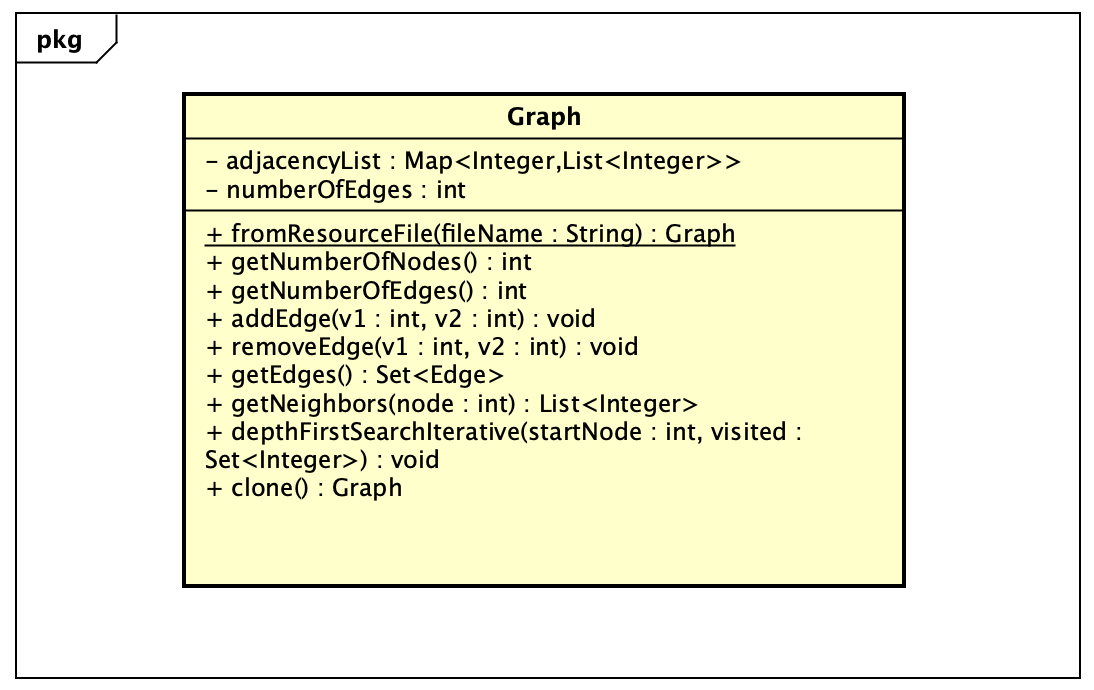
\includegraphics[width=0.6\textwidth]{figuras/graph-class.png}
	% Caption centralizada
% 	\captionsetup{justification=centering}
	% Caption e fonte 
	 \vspace{-0.2cm}
	\label{fig:figura1}
\end{figure}
\vspace{-0.5cm}

\subsection{\esp Identificação de Trajetos e Ciclos Eulerianos}

Além da estrutura do grafo, foi criada a classe \texttt{FleuryEulerTourFinder}, que é responsável por receber o grafo desejado e identificar possíveis trajetos ou ciclos eulerianos. A identificação é realizada utilizando um dos métodos de identificação de pontes, que é passado como um objeto do tipo \texttt{BridgeIdentifier} ao método construtor da classe, junto ao grafo desejado.

Inicialmente, a classe \texttt{FleuryEulerTourFinder} faz um clone do grafo enviado por parâmetro, sendo esse novo grafo um auxiliar, o qual terá as suas arestas removidas à medida que o trajeto euleriano é encontrado.

Em seguida, é executado o método \texttt{find()}, o qual dá início à busca pelo trajeto euleriano. O processo começa ao identificar um vértice inicial (\texttt{u}), sempre dando preferencia por vértices de grau impar, uma vez que o trajeto semi-euleriano precisa começar em um vértice de grau ímpar. O algoritmo, então, percorre o grafo, removendo arestas enquanto constrói o trajeto em \texttt{eulerTour}. Para realizar esse processo, chama o método auxiliar \texttt{getEulerTour(Integer)}, que explora o grafo a partir do vértice inicial e encontra o trajeto euleriano.

Durante o percurso, cada aresta é verificada pelo método \texttt{isBridge()}, da classe BridgeIdentifier, que determina se a aresta atual é uma ponte e, portanto, se sua remoção comprometeria a conectividade do grafo. 

A classe também conta com o método \texttt{classify()}, responsável por verificar se o grafo é euleriano, semi-euleriano ou não eureleriano.

 Tal fato pode ser vizualizado na figura \ref{fig:figura2}. 
% Figura
\begin{figure}[ht]
	\centering	
	\caption[\hspace{0.1cm}Grafo.]{Classe FleuryEulerTourFinder}
	\vspace{-0.4cm}
	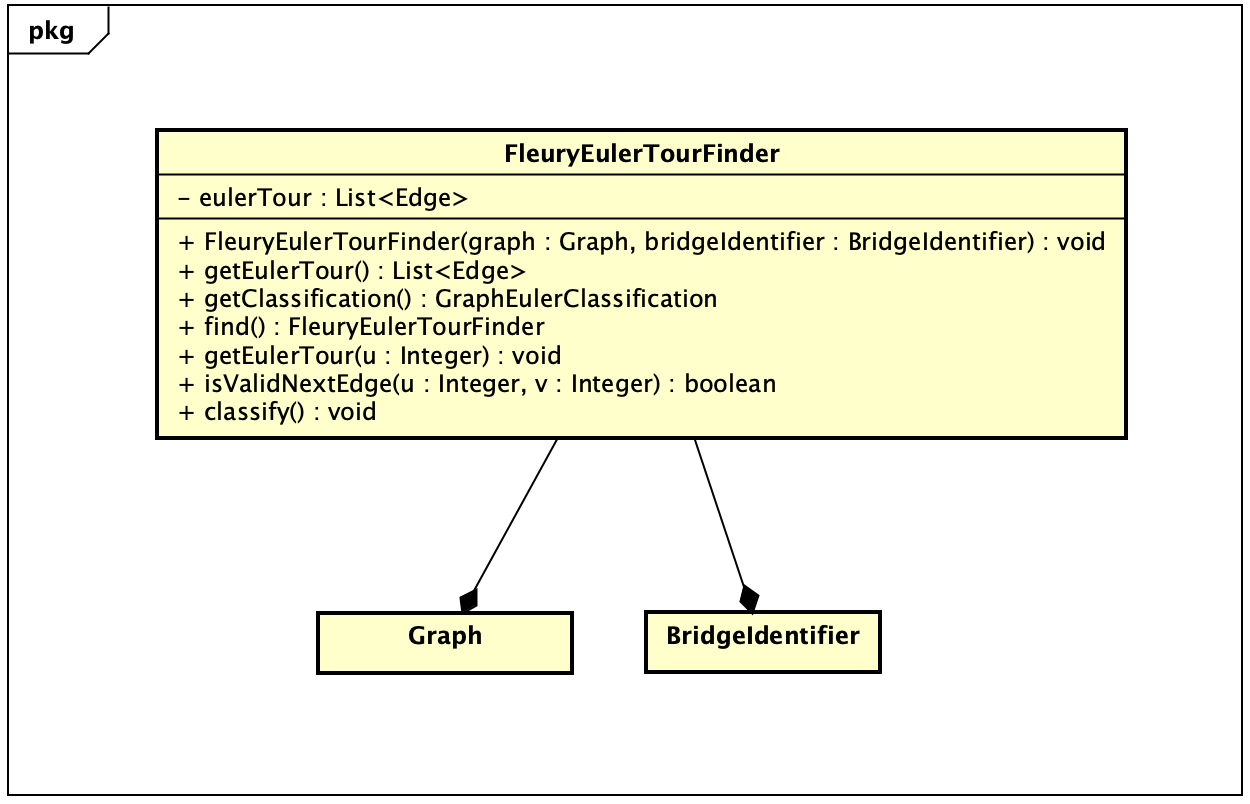
\includegraphics[width=0.6\textwidth]{figuras/fleury-euler-tour-finder-class.png}
	% Caption centralizada
% 	\captionsetup{justification=centering}
	% Caption e fonte 
	 \vspace{-0.2cm}
	\label{fig:figura2}
\end{figure}
\vspace{-0.5cm}


\subsection{\esp Identificação de Pontes}
As classes responsáveis pela identificação das pontes implementam a classe abstrata \texttt{BridgeIdentifier}, permitindo a fácil troca entre diferentes abordagens para a identificação de pontes, como os métodos \textit{Naïve} e \textit{Tarjan}, sem a necessidade de modificações no código. Tal fato pode ser visualizado na figura \ref{fig:figura3}.

% Figura
\begin{figure}[ht]
	\centering	
	\caption[\hspace{0.1cm}Grafo.]{Hierarquia de Classes BridgeIdentifier}
	\vspace{-0.4cm}
	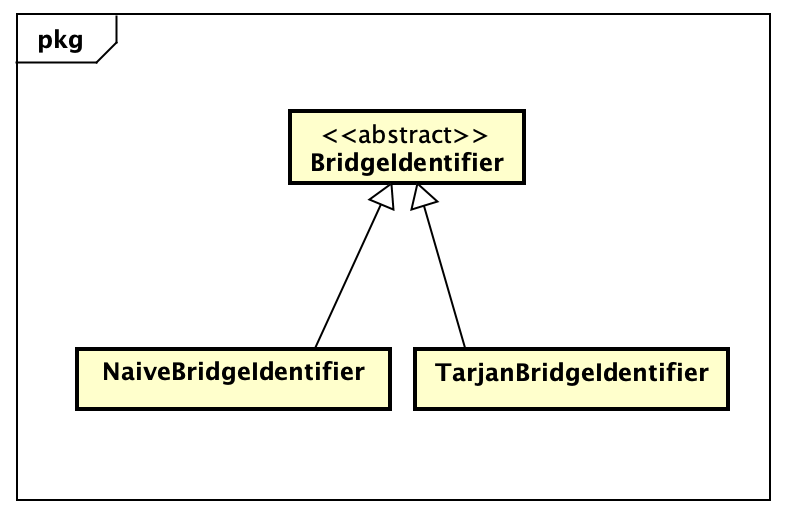
\includegraphics[width=0.6\textwidth]{figuras/bridge-identifier-hierarchy.png}
	% Caption centralizada
% 	\captionsetup{justification=centering}
	% Caption e fonte 
	 \vspace{-0.2cm}
	\label{fig:figura3}
\end{figure}
\vspace{-0.5cm}



\subsubsection{\esp Naïve}

A classe \texttt{NaiveBridgeIdentifier} identifica pontes no grafo utilizando o método \texttt{isBridge()}. Esse método realiza a identificação de pontes removendo temporariamente a aresta selecionada e, em seguida, chamando o método \texttt{isConnected()} no grafo. O método \texttt{isConnected()} executa uma busca em profundidade (DFS) para verificar se todos os vértices ainda podem ser alcançados, mesmo com a remoção da aresta. Caso algum vértice fique inacessível, a aresta removida é identificada como uma ponte, pois sua ausência desconecta o grafo.

\subsubsection{\esp Tarjan}

O algoritmo implementado na classe \texttt{TarjanBridgeIdentifier} visa identificar as pontes de um grafo utilizando a técnica de busca em profundidade (DFS) modificada.

A função principal, \texttt{isBridge()}, recebe um grafo e uma aresta como entrada. Para verificar se essa aresta é uma ponte, o algoritmo executa uma busca DFS começando a partir do vértice inicial da aresta. Durante a execução da DFS, o algoritmo mantém dois arrays auxiliares: \texttt{disc[]}, que armazena o tempo de descoberta de cada vértice, e \texttt{low[]}, que armazena o menor tempo de descoberta de um vértice alcançável a partir do vértice atual ou de seus descendentes.

Se, ao visitar um vértice \(v\), for encontrado um vértice \(u\) (vértice pai de \(v\)) tal que \texttt{low[v] > disc[u]}, então a aresta entre \(u\) e \(v\) é identificada como uma ponte, pois a remoção dessa aresta desconectaria o grafo.

O algoritmo usa duas pilhas para realizar a DFS de forma iterativa: uma pilha para armazenar os vértices a serem visitados (\texttt{stack}) e outra para armazenar os iteradores dos vizinhos de cada vértice (\texttt{adjStack}).



\subsection{\esp Testes}

Para a realização dos testes e obtenção dos resultados, foram gerados automaticamente diferentes grafos não direcionados, incluindo grafos Eulerianos, semi-Eulerianos e não Eulerianos, com tamanhos variando entre 100, 1.000, 10.000 e 100.000 vértices. Essa variação permitiu uma avaliação abrangente dos resultados dos métodos de identificação de pontes em grafos, possibilitando uma análise comparativa de desempenho entre as abordagens.

A criação dos grafos foi automatizada através do arquivo \texttt{generate\_graphs.py}. O código gera os três tipos de grafos: um ciclo fechado para grafos Eulerianos, um caminho com duas arestas extras para semi-Eulerianos e um caminho com múltiplas arestas extras para não Eulerianos. Cada grafo gerado é salvo em arquivos de texto, com nomes que indicam seu tipo e tamanho.

\section{\esp Resultados}

Para a obtenção dos resultados, o método \textit{Fleury} foi executado cinco vezes para cada grafo criado, com o tempo de execução de cada tentativa registrado em milissegundos. Em seguida, calcular-se-á a média aritmética desses tempos, proporcionando uma estimativa mais precisa do desempenho. Esse procedimento foi  realizado utilizando dois métodos distintos para a identificação de pontes: o método \textit{naïve} e o método \textit{Tarjan}.


Após a execução de ambos os métodos, os tempos médios de execução serão comparados, permitindo uma análise detalhada das diferenças de eficiência e desempenho entre as duas abordagens.


\begin{table}[htb]
	\centering
	\caption{\hspace{0.1cm} Tempo Médio de Execução dos Grafos Eulerianos Usando o Método Naïve para Identificação de Pontes }
	\vspace{-0.3cm} % espaço entre título e tabela
	\label{tab:tempo_execucao_naive}
	% Conteúdo da tabela
	\begin{tabular}{l|c|c}
    \hline
    \textbf{Grafo} & \textbf{Tempo Total (ms)} & \textbf{Média Aritmética (ms)} \\
    \hline
     eulerian\_100\_graph & 46 & 9 \\
     eulerian\_1000\_graph & 566 & 113 \\
     eulerian\_10000\_graph & 116610 & 23322 \\
     eulerian\_100000\_graph & 5x & x > 7200000 \\
    \hline
 \end{tabular}
 	\vspace{.1cm}  % espaço entre tabela e fonte
	\small
	% Fonte
	{\footnotesize\\ \textbf{Fonte: Dados obtidos pelo autor}}
\end{table}

\begin{table}[htb]
	\centering
	\caption{\hspace{0.1cm} Tempo Médio de execução dos grafos Eulerianos utilizando o método de Tarjan para identificação de pontes}
	\vspace{-0.3cm} % espaço entre título e tabela
	\label{tab:tempo_execucao_fleury}
	% Conteúdo da tabela
	\begin{tabular}{l|c|c}
    \hline
    \textbf{Grafo} & \textbf{Tempo Total (ms)} & \textbf{Média Aritmética (ms)} \\
    \hline
     eulerian\_100\_graph & 40 & 8 \\
     eulerian\_1000\_graph & 390 & 78 \\
     eulerian\_10000\_graph & 25252  & 5050 \\
     eulerian\_100000\_graph & 26262975 & 5252595 \\
    \hline
 \end{tabular}
 	\vspace{.1cm}  % espaço entre tabela e fonte
	\small
	% Fonte
	{\footnotesize\\ \textbf{Fonte: Dados obtidos pelo autor}}
\end{table}

\begin{table}[htb]
	\centering
	\caption{\hspace{0.1cm} Tempo Médio de Execução dos Grafos Semi-Eulerianos Utilizando o Método Naïve para Identificação de Pontes}
	\vspace{-0.3cm} % espaço entre título e tabela
	\label{tab:tempo_execucao_semi_eulerianos}
	% Conteúdo da tabela
	\begin{tabular}{l|c|c}
    \hline
    \textbf{Grafo} & \textbf{Tempo Total (ms)} & \textbf{Média Aritmética (ms)} \\
    \hline
     semi\_eulerian\_100\_graph & 44 & 8 \\
     semi\_eulerian\_1000\_graph & 844 & 168 \\
     semi\_eulerian\_10000\_graph & 127842 & 25380 \\
     semi\_eulerian\_100000\_graph & 5x &  x > 7200000 \\
    \hline
 \end{tabular}
 	\vspace{.1cm}  % espaço entre tabela e fonte
	\small
	% Fonte
	{\footnotesize\\ \textbf{Fonte: Dados obtidos pelo autor}}
\end{table}

\begin{table}[htb]
	\centering
	\caption{\hspace{0.1cm} Tempo Médio de Execução dos Grafos Semi-Eulerianos Usando o Método Tarjan para Identificação de Pontes}
	\vspace{-0.3cm} % espaço entre título e tabela
	\label{tab:tempo_execucao_semi_eulerianos_tarjan}
	% Conteúdo da tabela
	\begin{tabular}{l|c|c}
    \hline
    \textbf{Grafo} & \textbf{Tempo Total (ms)} & \textbf{Média Aritmética (ms)} \\
    \hline
     semi\_eulerian\_100\_graph & 42 & 8 \\
     semi\_eulerian\_1000\_graph & 378 & 75 \\
     semi\_eulerian\_10000\_graph & 25568 & 5113 \\
     semi\_eulerian\_100000\_graph & 26142521 & 5228504 \\
    \hline
 \end{tabular}
 	\vspace{.1cm}  % espaço entre tabela e fonte
	\small
	% Fonte
	{\footnotesize\\ \textbf{Fonte: Dados obtidos pelo autor}}
\end{table}

\begin{table}[htb]
	\centering
	\caption{\hspace{0.1cm} Tempo Médio de Execução dos Grafos Não-Eulerianos Usando o Método Naïve para Identificação de Pontes}
	\vspace{-0.3cm} % espaço entre título e tabela
	\label{tab:tempo_execucao_nao_eulerianos_naive}
	% Conteúdo da tabela
	\begin{tabular}{l|c|c}
    \hline
    \textbf{Grafo} & \textbf{Tempo Total (ms)} & \textbf{Média Aritmética (ms)} \\
    \hline
     non\_eulerian\_100\_graph & 49 & 9 \\
     non\_eulerian\_1000\_graph & 840 & 168 \\
     non\_eulerian\_10000\_graph & 101136 & 20227 \\
     non\_eulerian\_100000\_graph & 5x & x > 7200000 \\
    \hline
 \end{tabular}
 	\vspace{.1cm}  % espaço entre tabela e fonte
	\small
	% Fonte
	{\footnotesize\\ \textbf{Fonte: Dados obtidos pelo autor}}
\end{table}


\begin{table}[htb]
	\centering
	\caption{\hspace{0.1cm} Tempo Médio de Execução dos Grafos Não-Eulerianos Usando o Método de Tarjan para Identificação de Pontes}
	\vspace{-0.3cm} % espaço entre título e tabela
	\label{tab:tempo_execucao_nao_eulerianos_tarjan}
	% Conteúdo da tabela
	\begin{tabular}{l|c|c}
    \hline
    \textbf{Grafo} & \textbf{Tempo Total (ms)} & \textbf{Média Aritmética (ms)} \\
    \hline
     non\_eulerian\_100\_graph & 43 & 8 \\
     non\_eulerian\_1000\_graph & 436 & 87 \\
     non\_eulerian\_10000\_graph & 25829 & 5165 \\
     non\_eulerian\_100000\_graph & 30058036 & 6011607 \\
    \hline
 \end{tabular}
 	\vspace{.1cm}  % espaço entre tabela e fonte
	\small
	% Fonte
	{\footnotesize\\ \textbf{Fonte: Dados obtidos pelo autor}}
\end{table}

Os resultados apresentados nas Tabelas \ref{tab:tempo_execucao_naive}, \ref{tab:tempo_execucao_fleury}, \ref{tab:tempo_execucao_semi_eulerianos}, \ref{tab:tempo_execucao_semi_eulerianos_tarjan}, \ref{tab:tempo_execucao_nao_eulerianos_naive}, e \ref{tab:tempo_execucao_nao_eulerianos_tarjan} de tempo médio de execução mostram uma clara diferença de desempenho entre os métodos \textit{Naïve} e \textit{Tarjan} para a identificação de pontes em grafos Eulerianos, Semi-Eulerianos, e Não-Eulerianos. De maneira geral, o método \textit{Tarjan} se mostrou mais eficiente em todas as categorias de grafos, apresentando tempos de execução consistentemente menores em comparação ao método \textit{Naïve}. Por exemplo, no caso dos grafos \texttt{eulerian\_100000\_graph}, o método de \textit{Tarjan} levou apenas 5050 ms, enquanto o método \textit{Naïve} exigiu 23322 ms, conforme ilustrado nas Tabelas \ref{tab:tempo_execucao_naive} e \ref{tab:tempo_execucao_fleury}.

A razão para essa diferença de desempenho está diretamente relacionada às complexidades de ambos os métodos. O \textit{Método Naïve} apresenta uma complexidade de \textbf{O(V * E)}, o que implica que, à medida que o grafo aumenta em tamanho, o tempo de execução cresce de maneira significativamente mais rápida. Isso ocorre porque o algoritmo realiza uma busca para cada aresta, o que se torna muito custoso para grafos grandes.

Em contraste, o \textit{Método de Tarjan}, com complexidade \textbf{O(V + E)}, realiza a identificação de pontes em uma única varredura do grafo, sendo linear em relação ao número de vértices e arestas. Isso explica a superioridade do método \textit{Tarjan}, especialmente para grafos com 10.000 e 100.000 vértices, onde as diferenças de tempo se tornam evidentes, como mostrado nas Tabelas \ref{tab:tempo_execucao_naive}, \ref{tab:tempo_execucao_fleury}, \ref{tab:tempo_execucao_semi_eulerianos}, \ref{tab:tempo_execucao_semi_eulerianos_tarjan}, \ref{tab:tempo_execucao_nao_eulerianos_naive}, e \ref{tab:tempo_execucao_nao_eulerianos_tarjan}.


\section*{Conclusão}

Este estudo comparou os métodos \textit{naïve} e \textit{Tarjan} para a identificação de pontes em grafos, etapa essencial na execução do algoritmo de Fleury para encontrar trajetos e ciclos eulerianos. Os resultados evidenciam que o algoritmo de\textit{ Tarjan}, com complexidade \textbf{\(O(V + E)\)}, é significativamente mais eficiente que a abordagem \textit{naïve}, que opera em \textbf{\(O(V \times E)\)}. Para grafos maiores, o algoritmo de \textit{Tarjan} demonstrou maior praticidade, destacando a importância de algoritmos otimizados em aplicações da teoria dos grafos, como a otimização de rotas e análise de redes. Esta pesquisa reforça a necessidade de métodos eficientes na resolução de problemas baseados em grafos em diversos domínios.


% \subsection{\esp Trabalhos futuros}
% 
% Sugestões de estudos posteriores são ser adicionados subseção deste capítulo de conclusão.

%%%%%%%%%%%%%%%%%%%%%%%%%%%%%%%%%%%
%% FIM DO TEXTO
%%%%%%%%%%%%%%%%%%%%%%%%%%%%%%%%%%%

% \selectlanguage{brazil}
%%%%%%%%%%%%%%%%%%%%%%%%%%%%%%%%%%%
%% Inicio bibliografia
%%%%%%%%%%%%%%%%%%%%%%%%%%%%%%%%%%%

 \newpage
 \singlespace{
 \bibliographystyle{abntex2-alf}
 \bibliography{bibliografia}
 }

\end{document}